
A key property of a particle is how it decays into other particles. \gls{ATLAS}\footnote{A Toroidal LHC Apparatus} is a particle physics experiment at \gls{CERN}\footnote{The European organization for nuclear research} that searches for new particles and processes using head-on collisions of protons at extraordinarily high energies \cite{open}. In 2012, the ATLAS experiment claimed the discovery of a new particle, the Higgs boson. The discovery has a statistical significance of 5$\sigma$ which corresponds to a 1 in 3.5 million chance of the results being obtained purely due to chance. In essence, it denotes a very high confidence in the discovery. The Higgs awaited experimental evidence for over four decades, it was postulated by physicist Peter Higgs in 1964 \cite{higgs}. The existence of this particle provides support to the theory that a field permeates the universe through which fundamental particles acquire mass, a theory which is cardinal for the completeness of the Standard Model of particle physics. The proton-proton collisions in the ATLAS detector produce thousands of collision events per second. Each collision event can be summarised by numeric information represented by a vector of several dimensions. These represent the \textit{features} as in standard machine learning parlance. This thesis views the physics problem of identification of a Higgs decay from a machine learning perspective. The main objective of the thesis is to cast the problem as a binary classification problem and propose an algorithm that addresses the main challenge in the dataset, that of overlapping classes. 

The dataset used to train, cross-validate and test the algorithm proposed in this thesis is obtained from the CERN Open Data portal \cite{data}. The dataset used in this thesis is a modified version of the dataset physicists used in the ATLAS results made public in December 2013 in the CERN Seminar, \textit{ATLAS sees Higgs decay to fermions} \cite{fermions}.

\section{Organization of the thesis}

Chapter \ref{intro} introduces the goal of the problem in a physics context. Chapter \ref{mlhep} provides a discussion of how machine learning techniques are typically used in experimental physics by citing some published approaches. The third chapter \ref{formal} provides a mathematical description of the problem concluding with a summary of the challenges inherent in the machine learning incarnation of the problem. Chapter \ref{formal} also introduces the Approximate Median Significance (\gls{AMS}) metric which is a physics inspired metric used to assess the performance of a binary classifier designed for the task of separating signal from background. It sheds some light on the motivation for the statistical formula of the metric. Chapter \ref{performance} contrasts the AMS metric with standard machine learning metrics in classification tasks. Chapter \ref{ad} introduces the theory behind meta algorithms and Chapter \ref{results} contains performance results of a proposed algorithm on the ATLAS Higgs dataset in terms of the AMS. Chapter \ref{concl} has concluding remarks.

\section{Physics Background} 

Each generation of high energy physics experiments is more demanding in terms of multivariate analysis. Machine learning - known in the physics circles as multivariate analysis played a key role in the Higgs analysis that led to the 2012 discovery. In this section we provide an accessible overview to some of the physics concepts needed to understand the primary data which serve as features to the machine learning model. 

\subsection{Decay Channel}

Particles produced in the proton-proton collisions are unstable and decay almost instantaneously into a cascade of lighter particles. These sets of second order and third order particles represent a \textit{decay} channel or a \textit{decay} product. The surviving particles which live long enough for their properties to be measured by the detector are called \textit{final-state} particles. 

The Higgs boson (H) is unstable and is known to have five main experimentally accessible decay channels. Each occurs which a certain probability, this is called the branching ratio. The branching ratios of the Higgs boson depend on its mass and are precisely predicted in the standard model. The SM predicts branching ratios as a function of the Higgs mass. For a SM Higgs of mass 125 GeV, the first-order decay products and their respective probabilities are :

\begin{center}

\scalebox{0.7}{
\begin{tabular}{|l|l|l|l|}
\hline
\rule[-1ex]{0pt}{2.5ex} Decay Channel & Description & Branching Ratio & Status \\ 
\hline 
\rule[-1ex]{0pt}{2.5ex}  $H \rightarrow b\bar{b}$ & b quark and its anti-quark & 0.577 & predicted \\ 
\rule[-1ex]{0pt}{2.5ex} $ H \rightarrow \tau^{+} \tau^{-} $ & $\tau$ lepton and its anti-particle & 0.063 & predicted \\ 
\rule[-1ex]{0pt}{2.5ex} $ H \rightarrow \gamma\gamma $ & di-photon channel & 0.0023 & observed\\ 
\rule[-1ex]{0pt}{2.5ex} $ H \rightarrow W^{+}W^{-} $ & W boson and its anti-particle & 0.215 & observed\\ 
\rule[-1ex]{0pt}{2.5ex} $ H \rightarrow Z^{0}Z^{0} $ & A pair of Z bosons &  0.026 & observed\\
\rule[-1ex]{0pt}{2.5ex} & Various other decays &   & predicted\\
\hline
\end{tabular}} 
\end{center}
 
The analysis presented in this thesis concerns the $H \rightarrow \tau^{+} \tau^{-}$ channel which characterize the signal events in the dataset. This is explained further in section \ref{taudecay}.

The measured momenta of final state particles are primary information used to identify a Higgs decay.

The ATLAS detector measures three properties of each of the detectable final state particles, they are :

\begin{enumerate}[noitemsep]
\item{The \textit{type} (lepton, hadronic tau, jets)} \item{The \textit{energy}, $E$}
\item{The \textit{3D direction} expressed as a vector $(p_{x}, p_{y}, p_{z})$}
\end{enumerate}

\textit{Note:} Neutrinos are not among the detected final-state particles but appear in the final state. The feature associated with the undetected neutrinos is the \textit{missing transverse momentum}. The concept of transverse momentum deserves a detailed explanation which is provided in section \ref{missing}.

\begin{figure}[ht]
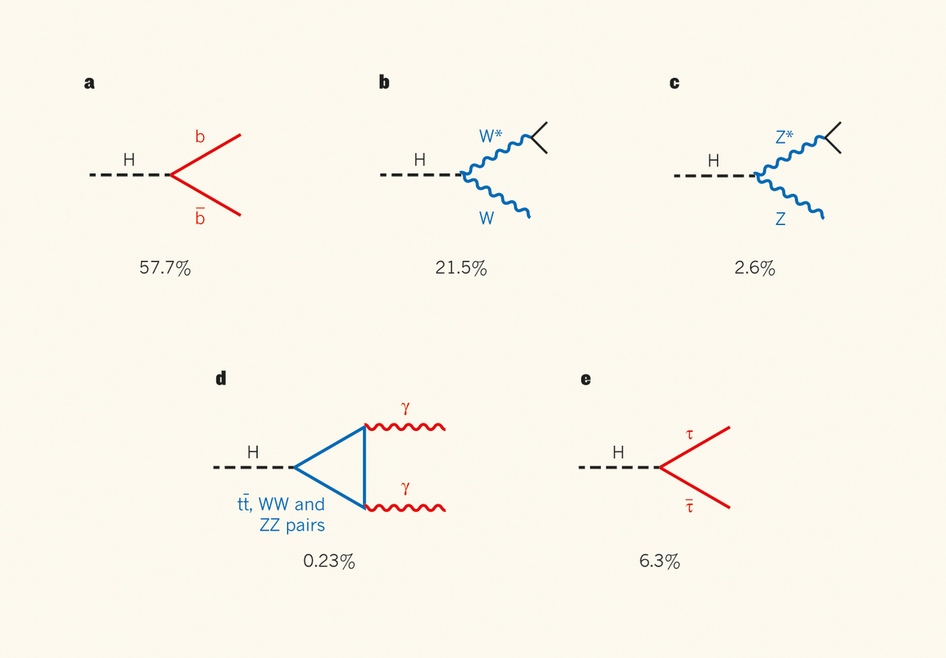
\includegraphics[scale=0.43,width=\textwidth]{images/higgs_branching.jpg}
\caption{Dominant decay modes for the Higgs boson. Adapted from \cite{hdecay}.}
\end{figure}

\subsection{Invariant Mass}

The mass of a particle is an intrinsic property of a particle, further by the law of conservation of energy and momentum the mass of a particle is equivalent to the mass of its decayed products each of which can be represented by their 4-momentum ($p_{x},p_{y},p_{z},E$) where $E$ is energy. For example, a particle $\chi$ decays into two final state particles $a$ and $b$ whose kinematics are captured in the detector. By conservation of energy and momentum, $$E_{\chi} = E_{a} + E_{b}$$ $$\overrightarrow{p_{\chi}} = \overrightarrow{p_{a}} + \overrightarrow{p_{b}}$$

The sum of energies and momenta of particles $a$ and $b$ should resolve to give the energy and momenta of the parent particle. The mass of the parent particle is then calculated as, 

\begin{equation}
m_{\chi} = \sqrt{E_{\chi}^2 - \overrightarrow{p_{\chi}}^2} 
\label{mass_invariant}
\end{equation}

Equation \ref{mass_invariant} originates from the energy-momentum relation,

\begin{equation}
E^2 = p^2c^2 + m^2c^4
\end{equation}

relating a particle's intrinsic rest mass $m$, energy $E$ and momentum. In natural units where $c=1$ this simplifies to,

\begin{equation}
E^2 = p^2 + m^2 
\end{equation}

(See Appendix \ref{App})

When a particle decays into lighter particles, its mass before the decay can be calculated from the energies and momenta of the decay products. The inferred mass is independent of the reference frame in which the energies and momenta are measured, so the mass is called \textit{invariant}.

This is the \textit{invariant mass principle} in classical mechanics. It holds for all particles including the Higgs boson and can be generalised to more than two final states and holds in every intermediate stage of decay.   

\subsection{Missing transverse momentum}
\label{missing}

In the 3D reference frame of ATLAS, the $z$-axis points along the horizontal beam line. The $x-y$ plane is perpendicular to the beam axis and is called the \textit{transverse plane}. The transverse momentum is the momentum of an object transverse to the beam axis (or in the transverse plane). The law of conservation momentum promotes the idea of \textit{missing transverse momentum}.

The law of conservation momentum states that the total momentum is conserved in a closed system before and after a collision. We do know that the initial momentum in the plane transverse to the beam axis is zero. Hence, the sum of transverse momentum of all particles (detected + undetected) post-collision should be zero. 

The missing transverse momentum is defined as, $E_{miss}^{T} =  - \sum_{i} \vec{p_{T}}(i) $ for visible particles $i$ where $\vec{p_{T}}$ is the transverse momentum. Essentially, a net momentum of outgoing visible particles indicates missing transverse momentum attributed to particles invisible to the detector, like neutrinos. We know that the final state events consists of neutrinos and it is reasonable to estimate that they make up a lot of the missing transverse momentum.

\subsection{Tau Decay}
\label{taudecay}

In the original discovery the Higgs was seen decaying into $\gamma\gamma$, $W^{+}W^{-}$ and $Z^{0}Z^{0}$. The $H \rightarrow \tau^{+} \tau^{-}$ channel is particularly interesting as it hasn't been experimentally verified .i.e. its statistical significance is not yet at 5$\sigma$. 

It is important to understand what makes this specific decay channel hard to observe. There are two main reasons for this :

\begin{enumerate}

\item The decay into two taus is not a unique channel, in fact the Z boson can also decay into two taus, further this happens a lot more frequently than the Higgs. The precise mass of the Z boson is 91 GeV, since this is not very far from the mass of the target Higgs (125 GeV), the two decays produce events which have very similar signatures and this prevents a clean separation of the parent candidate.

\item Taus are heavy and unstable, they decay instantaneously. Their dominant decay modes involve neutrinos and the presence of these undetectable particles in their decay make it difficult to reconstruct the parent mass on an event by event basis.
\end{enumerate}

The three dominant channels of $\tau$ decay are: 
\begin{enumerate}[noitemsep]
\item{$\tau \rightarrow e^{-}\nu_{e}\nu_{e}$} [an electron and two neutrinos]
\item{$\tau \rightarrow \mu^{-}\nu_{\mu}\nu_{\mu}$} [a muon and two neutrinos]
\item{$\tau \rightarrow$  $\tau$-hadron and $\nu_{\tau}$ [a tau-hadron and a neutrino]}
\end{enumerate} 
The data underlying the results in this thesis focuses on the $H \rightarrow \tau^{+} \tau^{-}$ decay channel where the signal events indicate a Higgs decay to two taus and background events are characterized by the same tau-tau channel but from the decay of a non-Higgs particle.

%\subsection{\texorpdfstring{$H \rightarrow \tau^{+} \tau^{-}$}{} decay : A binary classification framework}
%\label{taudecay2}
%
%As mentioned in section \ref{taudecay} the Higgs discovery in 2012 was confirmed only in three out of the five decay channels of the Higgs. The exploration of the $H \rightarrow \tau^{+} \tau^{-}$ channel is experimentally hard because the decay signature of this channel is very similar to several other background decays, like the abundant Z boson decay. 
%
%In order to promote collaboration between high energy physicists and machine learning experts a challenge (HiggsML challenge for short) was organized by a small group of ATLAS physicists. It was hosted by Kaggle at \url{https://www.kaggle.com/c/higgs-boson} from May to September 2014. 
%The subject of the challenge was to view the problem of identifying the 
%$H \rightarrow \tau^{+} \tau^{-}$ channel as a binary classification problem. Properties of collision events were preprocessed and presented as numerical vectors which serve as feature inputs to the machine learning algorithm. Fundamentally, the problem is to classify events as  a signal (a $H \rightarrow \tau^{+} \tau^{-}$ decay) or background (a non-Higgs decay). The only dataset provided for the challenge was a set of 250K events with 30 features per event. 
%
%Post the completion of the challenge a larger data-set consisting of 800K labelled events (signal/background) was released on the CERN Open Data Portal. Apart from the 30 features per event ATLAS provided an additional attribute which helped divide the data into relevant chunks highlighting their role in the machine learning analysis, each event belonged to either the training set (250K events), the validation set (100K events) or the testing set (450K events). This thesis uses this larger dataset.
%
%The goal statement released by the ATLAS collaboration was - \textit{``to explore the potential of advanced classification methods to improve the statistical significance of the $H \rightarrow \tau^{+} \tau^{-}$ channel''}\cite{rm}.

\begin{figure}
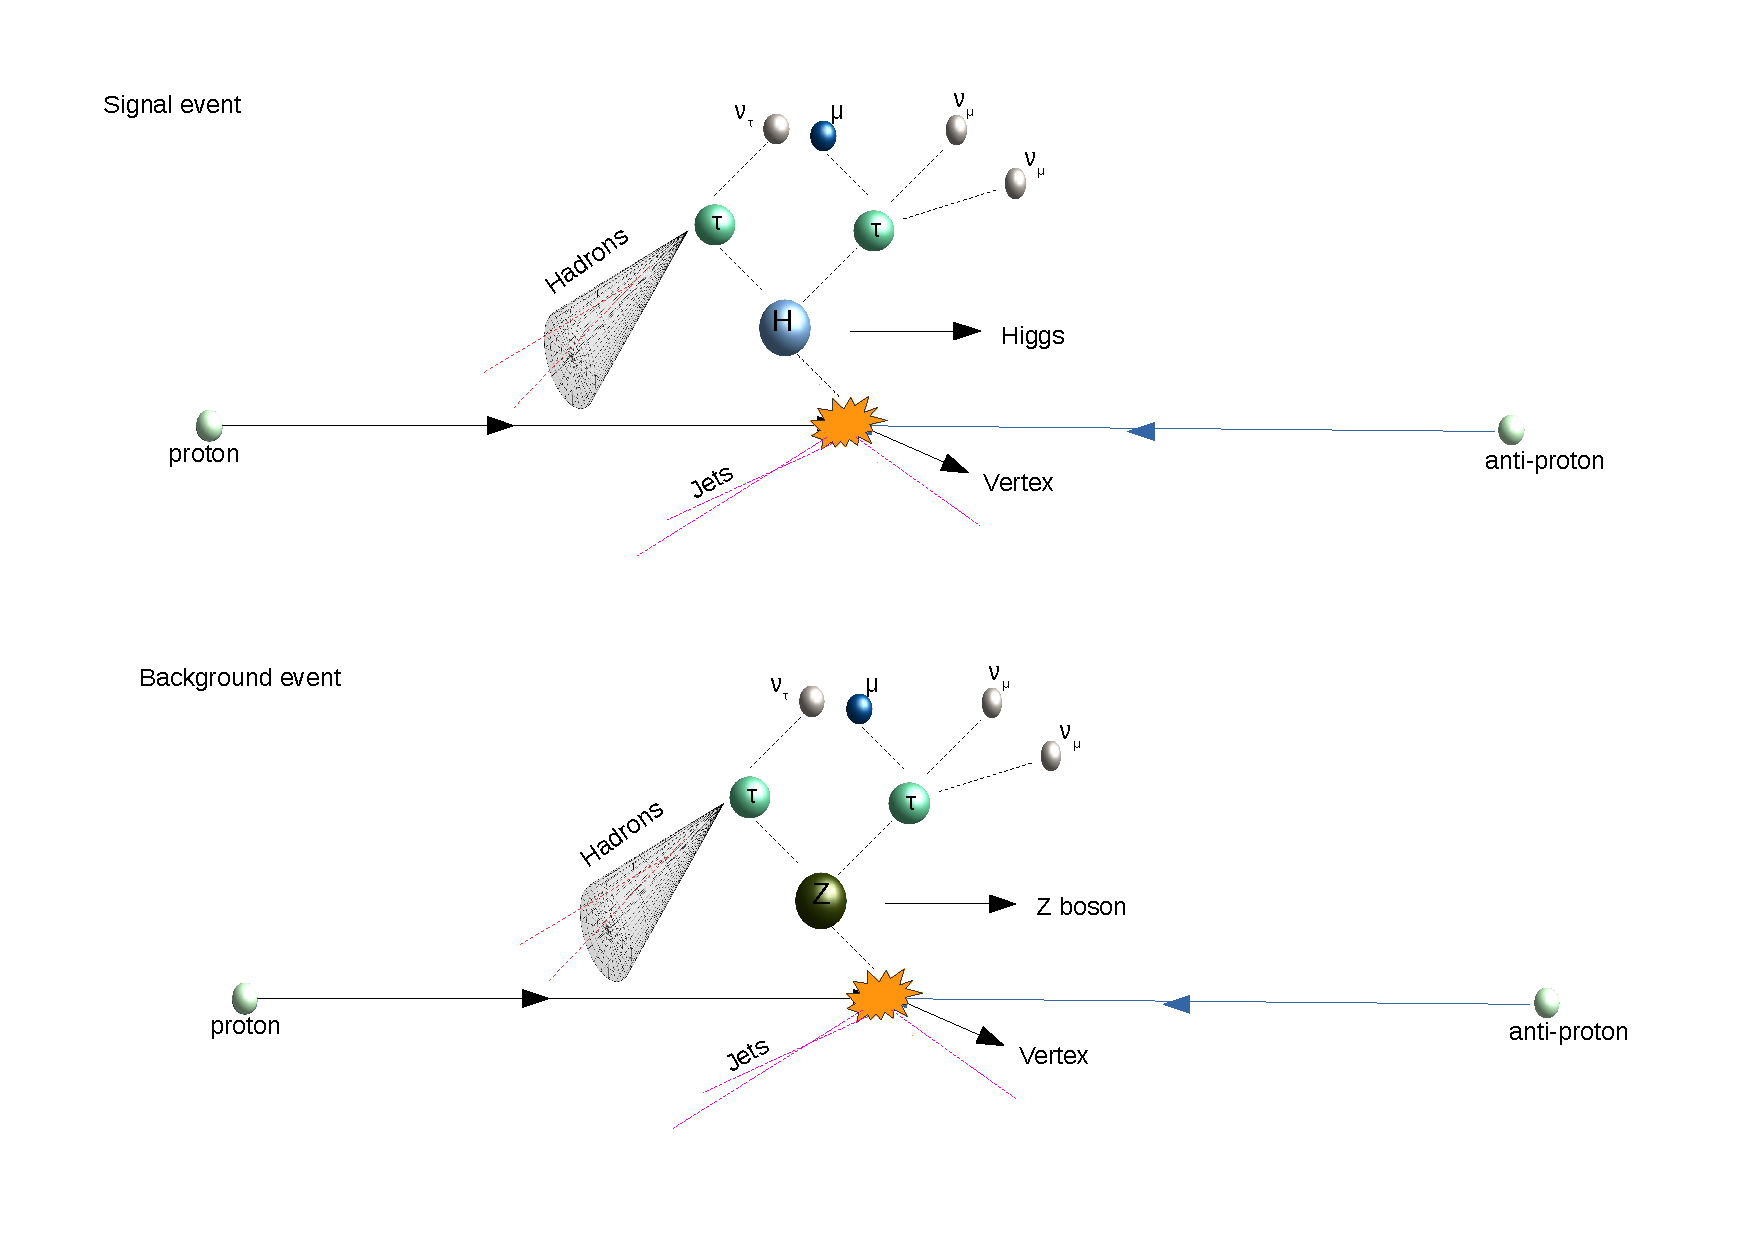
\includegraphics[width=\textwidth]{images/higgs_decay.pdf}
\caption{H and Z decay channel with similar signature}
\end{figure}

\subsection{Collider events}

The LHC collides bunches of protons every 50 nanoseconds at four interaction points. Each bunch crossing yields more than 20 proton-proton collisions on average. The average number of collisions per bunch crossing is between 10 and 35 depending on the conditions inside the collider. The colliding protons produce a small firework in which new particles are released as a result of the kinetic energy of the protons. An online trigger classifier system discards a vast majority of bunch collisions which contain uninteresting events, this decreases the event rate from 20,000,000 to about 400 per second. The selected 400 events are saved on disk producing about 1 billion events and three petabytes of raw data per year.   

\subsection{Simulated Data}

The dataset used in this thesis is a simulated dataset constructed by ATLAS physicists. Because the problem is the discovery of new phenomenon, labelled samples of actual signal events are not available. Hence, classifiers cannot be trained on real accelerator data. Instead, the data are drawn from elaborate simulators of the accelerator which generate events following the rules of the Standard Model and take into account noise and other artefacts. The simulators are sophisticated models that capture the best current understanding of the physical processes and have been thoroughly verified using data from previous accelerators. The classifiers are trained and validated on such data before they are applied to real unseen data with no class labels.   

\subsection{Experimental search process}
\label{esp}

The Higgs ($H$) is unstable and decays almost instantaneously into lighter particles, further its occurrence is rare. In order to create conditions for a $H$ decay two beams of protons are accelerated to energies close to the speed of light and collided inside a particle detector. The detector cannot directly observe $H$ but registers properties of the decay products. The reconstructed decay may match a possible $H$ decay but this is not enough to establish if $H$ was actually created. Many parent particles could have produced similar decay signatures. This complicates direct analytical inference. However, the SM predicts the likelihood of decay signatures of each know process. Hence, if the detector detects more decay signatures consistently matching a $H$ decay than would have been expected if $H$ did not exist, then that would be strong evidence that $H$ does exist. More precisely, the excess has to be atleast 5$\sigma$ i.e., the observed decays need to be more than 5 standard deviations away from the expectation if there was no new particle, in this case no Higgs.  

The question is really that of statistical significance, because the occurrence of $H$ is so rare and a high threshold of statistical significance needs to be reached a large number of collision events need to be analysed to ensure that correct conclusions are being drawn.  

The 4th July, 2012 announcement claiming the Higgs discovery under the di-photon channel entailed sifting through over 300 trillion ($3$x$10^{4}$) proton-proton collisions using the world's largest computing grid at the Large Hadron Collider at CERN. 


\begin{sidewaysfigure}
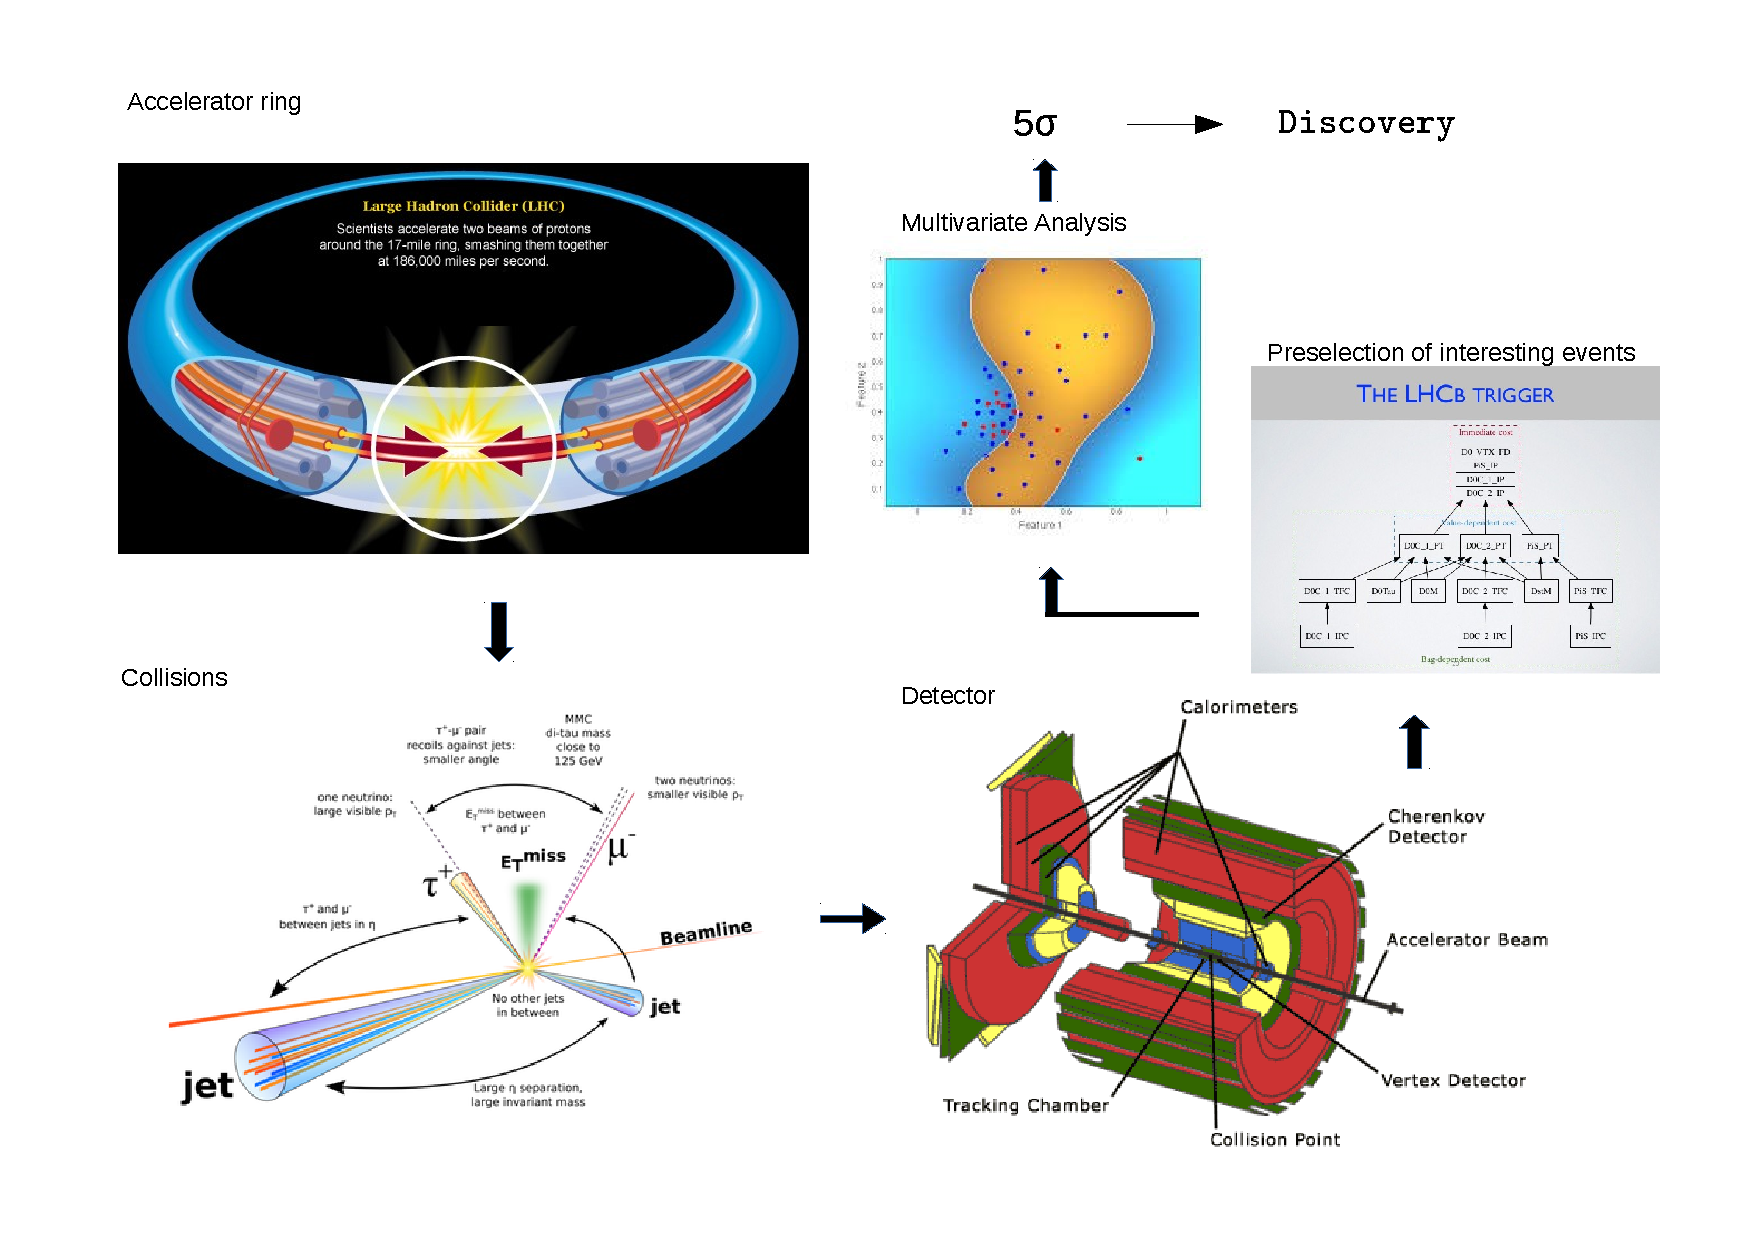
\includegraphics[width=\textwidth]{images/discovery.pdf}
\caption{Illustration of experimental search. Adapted from \cite{detector} and \cite{lhcb}.}
\end{sidewaysfigure}
